\documentclass[conference]{IEEEtran}

\usepackage[british]{babel}
\usepackage[hyphens]{url}
\usepackage{graphicx}
\usepackage[noadjust]{cite}
\usepackage[pdftex,colorlinks=true]{hyperref}

\begin{document}
\bstctlcite{IEEEexample:BSTcontrol}

% still not happy with the title...
\title{``Can I Implement Your Algorithm?'':\\ A Model for Benchmarking Research Software}

% author names and affiliations
% use a multiple column layout for up to three different
% affiliations
\author{\IEEEauthorblockN{Tom Crick}
\IEEEauthorblockA{Department of Computing\\
Cardiff Metropolitan University\\
Cardiff, UK\\
Email: {\url{tcrick@cardiffmet.ac.uk}}}
\and
\IEEEauthorblockN{Benjamin A. Hall}
\IEEEauthorblockA{Microsoft Research\\
Cambridge, UK\\
Email: {\url{benhall@microsoft.com}}}
\and
\IEEEauthorblockN{Samin Ishtiaq}
\IEEEauthorblockA{Microsoft Research\\
Cambridge, UK\\
Email: {\url{samin.ishtiaq@microsoft.com}}} }

\maketitle

\begin{abstract}
Abstract here...
\end{abstract}

\IEEEpeerreviewmaketitle

\section{Introduction}

Marc Andreessen famously said in 2011 that ``software is eating the
world''~\cite{andreessen:2011}. It's true: we clearly live in a
computational world, with our everyday interactions, entertainment,
books, shopping, keys, transportation, \dots\ are all heavily dependent on (or
replaced by) software.

This is also true in science and engineering. A 2012 report by the
Royal Society stated that computational techniques have ``{\emph{moved
on from assisting scientists in doing science, to transforming both
how science is done and what science is
done}}''~\cite{rssaaoe:2012}. New experiments, simulations, models,
benchmarks, even proofs cannot be done without software. And this
software does not consist of simple use-once, throw-away scripts;
scientific software repositories contain thousands, perhaps millions,
of lines of code and they need to be actively maintained. More
importantly, with reproducibility being a fundamental tenet of
science, they need to be re-useable.

However, if we want to be truthful about this, then the scientific
literature related to software tools often do not appear to be
adhering to the rules themselves. There are numerous
examples~\cite{beck-et-al:2005,prosser:2012}; how many of them are
reproducible? How many explain their experimental methodologies, in
particular the basis for their benchmarking? Can we build the
code?~\cite{collberg-et-al:2014} We, the authors, are as guilty as
anyone in the past, where we have succumbed to publishing
papers~\cite{crick-et-al:2009,Berdine2011SLAyer} with benchmarks and
promises of code to be released in the near future.

There are many reasons why the wider scientific community is in this
state. We are experiencing significant changes in academic
dissemination and publication, especially the open access movement,
with new models being
proposed~\cite{stodden-et-al:2013,fursin+dubach:2014}.  There are
numerous non-technical impediments to making software maintainable and
re-useable, too. The pressure to ``make the discovery'' and publish
quickly disincentivises careful software development. Releasing
code prematurely is often seen to give your competitors an
advantage. But we should be shining light into ``black
boxes''~\cite{morin-et-al:2012}.

Things can and should be much better. In this short paper, we
present a call to action with a small set of recommendations which we
hope will lead to better, more sustainable, more re-useable software,
to move towards an imagined future practice of software development
and usage in science and engineering.  The basis for many of these
recommendations is the basic scientific tenet of openness. There has
been previous work in this
area~\cite{sim-et-al:2003,chirigati-et-al:2013}, as well as a range of
manifestos for reproducible research and community initiatives, such
as cTuning~\footnote{\url{http://ctuning.org/}} and the Recomputation
Manifesto~\cite{gent:2013}~\footnote{\url{http://www.recomputation.org/}},
as well as recommendations on where to publish
software~\footnote{\url{http://www.software.ac.uk/resources/guides/which-journals-should-i-publish-my-software}}.


\section{Can I implement your algorithm?}

Reproducibility is a basic tenet of good Science. Yet many
descriptions of algorithms are too high-level, too obscure, too
hand-wavey to allow an easy implementation by a third party. A line in
the algorithm might say: ``We pick an element from the frontier set''
but which element do you pick? Will the first one do? Why will any
element suffice? Sometimes the author would like to give more details
but the space limit on papers is a hard one. Sometimes the authors
description in-lines many other algorithms or data structures that
perhaps only the author is familiar with.

We recommend here that a paper must describe the algorithm in such a
way that it is implementable by any reader of that algorithm. This is
subjective, of course. So, we also recommend that good scientific
conferences have a special track for papers that only re-implement
past papers' algorithms, techniques, or tools.


\section{Set the code free} 

There can be no better proof that your algorithm works, than if you
provide the source code of an implementation. Software development is
hard, but sharing and using others code is relatively easy.

A long time ago, Richard Stallman imagined that all code would be free
and we'd make our money by consulting on the code.
Surprisingly/amusingly, this is the case for a significant part of the
computing industry now. There are, of course, hard commercial
pressures for keeping code closed-source. Even in the scientific
domain, scientists and their collaborators may wish to hold onto their
code as a competitive advantage, especially if there exist larger
competitors who could use the available code to ``reverse scoop'' the
inventors, and so to charge into a promising new area opened by the
inventors.

Closed source is one thing. Licenses that deny the user from viewing,
modifying, or sharing the source are one thing. There are however even
licences on widely adopted tools like GAUSSIAN~\cite{Giles2004} that
prohibit even analyzing software performance and behaviour.
 
There is little doubt that, if science wants to be open and free,
then the code that underlies it too wants to be open and free. Code
that is available for browsing, modifying, and forking facilitates
testing and comparison, and promotes competition.

We recommend that code be published under an appropriate open source
license~\cite{osl}; BSD and Apache are good, flexible ones.%, though
IANAL.  A wide variety of licenses exist for molecular dynamics
software, with different degrees of openness
(GROMACS=LGPL~\cite{Hess2008} ,CHARMM/CHARMm and
Desmond=Academic/Commercial software
licences~\cite{Brooks2009,Bowers2006}, Amber and NAMD=custom open-like
licences). Z3 is an example from the verification area: the code
itself is not open source, but the MSR-LA that allows the source code
to be read, copied, forked for academic use, provides scholars in the
field much more than before~\cite{deMoura2012Z3open}.

Ultimately: set the code free. Put it on a place like GitHub, where it
is easy to fork and share. You should embrace the spirit of CRAPL
academic-strength open source
license~\footnote{\url{http://matt.might.net/articles/crapl/}} and
publish your code -- it is good enough~\cite{barnes:2010}.


\section{Be a better person}

If you have the skills and the experience, you can create better
software. We have seen the rise of initiatives, such as the Software
Carpentry~\footnote{\url{http://software-carpentry.org/}}, Software
Sustainability Institute~\footnote{\url{http://www.software.ac.uk/}}
and the UK Community of Research Software
Engineers~\footnote{\url{http://www.rse.ac.uk}} to cultivate
world-class research through software, develop software skills and
raise the profile of research software engineers.

Some scientists may not have had any formal, or even informal,
training in programming. Even basic training in software engineering
concepts like revision control, unit tests, etc can help improve the
quality of the software written enormously
http://philipwfowler.wordpress.com/2013/12/19/the-oxford-software-carpentry-boot-camp-one-year-on/
~\cite{Wilson2014}.  Interestingly, many of these concepts are taught
to computing undergraduates, but it could be argued that they are
taught at the wrong time of the engineers' careers, where the
importance of complex, long-running projects is not yet appreciated.

These are fundamental literacies for scientists and engineers: we
recommend that basic programming and computational skills are taught
as a core at undergraduate and postgraduate levels.


\section{Latin mass is better}

There really is no other scientific or technical field where its
participants can just make up a non-principled artefact like a
programming language so easily. In a way, it says how much a
``commons'' computer science is, that anyone and his dog can create a
new programming language or frameowrk or compiler. This has
advantages, and dis-advantages.

What is clear is that the use of a principled, high-level programming
language to write your software in, helps hugely with the
maintainability and robustness of the software. Such programming
languages impose constraints like types: you can never add a number
and a string is most basic example, but ML's functors provide
princpled ways of plugging in components with their implementations
completely hidden. Aggressive type checking avoids a subset of bugs
which can arise due to incorrectly written functions e.g. well
publicised NASA problems with a Mars orbiter
(http://www.cnn.com/TECH/space/9909/30/mars.metric.02/).
One example is a pressure coupling bug in GROMACS~\cite{Hess2008},
\url{http://redmine.gromacs.org/issues/14}, which arose due to the
inappropriate swapping of a pressure term with a stress tensor.  A
further extension of types, a concept called units of measure that is
implemented in languages such as F\#, can deal with these kinds of
bugs at compile time.
%[SI: Ben, can this be folded into the narrative above? Or does it need a separate para?]
Similarly, problems found using in house software for crystallography lead to 5
retractions \cite{Miller2006}, that arose due to a bug which inverted
the phases.

High level languages are often more readable than their
competitors. The ``density'' of a program is often seen to be a good
thing, but it's not always the case that a shorter Haskell program is
better to maintain than longer Python/C++ one. Nevertheless, what is
important is the readability of the code itself. A good example here
is from the world of automatic theorem proving: the SSReflect language
is much more readable than the original, standard Coq
language~\cite{GonthierZND13}. SSReflect uses mathematicians'
vernacular for script commands, allows reproducibility of automatic
proof checking because parameters are named rather than numbered,
etc. Even though these proof scripts are really only ever going to be
run by a machine, they seek to maintain the basic mathematical idea
that a proof should be readable by another mathematician.

\section{Test it to see}

Some models may be chaotic and influenced by floating point errors
(e.g. molecular dynamics), further frustrating testing. For example:
Sidekick is an automated tool for building molecular models and
performing simulations~\cite{Hall2014Sidekick}. Each system is
simulated from an different initial random seed, and under most
circumstances this is the only difference expected between
replicas. However, on a mixed cluster with both AMD and Intel
microprocessors on the nodes, the difference in architecture was found
to alter the number of water molecules added to each system by
one. This meant that the same simulation performed on different
architectures would diverge. Similarly, in a different simulation
engine, different neighbour searching strategies gave divergent
simulations due to the differing order in which forces were summed.

Despite these challenges to testing, unshared code is untestable.
Testing new complex scientific software is
difficult, as until the software is complete unit tests may not be
available. You should thus link from shared code -- shared code is
more test-able.

\section{Lineage} 

Research software is not just software -- it is the instantiation of
novel algorithms and data structures (or at least novel applications
of data structures). Thus, lineage is important: the code should
include links to papers publishing key algorithms and the
code should include explicit relationships to other projects on the
repository (i.e. {\emph{Project B}} was branched from {\emph{Project
A}}). This ensure that both the researchers and software developers
working upstream of the current project are properly credited,
encouraging future sharing and development. Remember, the people who
did the research are not necessarily the same people as the developers
and maintainers of the software, so it is important to reward both
appropriately with citations (a good way of doing this is the use of
CITATION
files~\footnote{\url{http://blog.rtwilson.com/encouraging-citation-of-software-introducing-citation-files/}}).


\section{YMMV}

\begin{figure}[!ht]
\centering
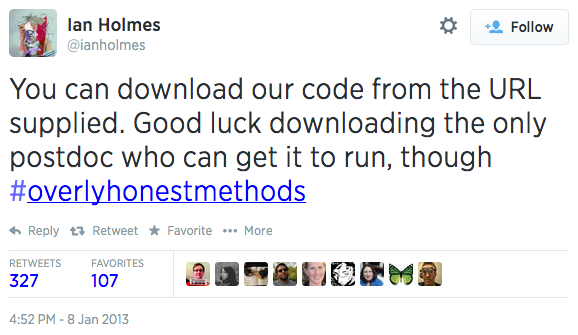
\includegraphics[width=\columnwidth]{overlyhonesttweet.png}
\caption{An \#overlyhonestmethod\newline [source: \url{https://twitter.com/ianholmes/status/288689712636493824}]}
\label{fig:overlyhonestmethod} 
\end{figure}

The tweet is Figure~\ref{fig:overlyhonestmethod} is funny because it
is so true. Often, the tool that the paper describes doesn't exist for
download. Or runs only on one particular platform. Or might run for
the author, for a while, but will bit-rot so soon that even the author
cannot compile it in two months time.

Providing the source code of the tool helps with this, of course. But
you must also provide details of \emph{how} you built and wrote the
software:
%
you should provide the compiler and build toolchain; 
%
you should provide builds tools/makefiles/ant/etc and build instructions; 
%
you should list or link to all non-standard packages and libraries that you use; 
%
you should note the hardware and OS used. 
%
This sounds like a lot of work, but GitHub APIs, CI, VMs and cloud can
make it easier; see Section~\ref{sec:Conclusion} at the end for more
on this.


\section{Forms of representation}


We often do not, and should not care, how things are stored on disk,
what their representations are. But a common, constrained, standard
representation is good for passing tests or models around between
different tools. A properly described representation, like the SMT-LIB
format for SAT Modulo Theory solvers~\cite{smtlib}, where both the
syntax and semantics are well understood, aids hugely in developing
tools, techniques, benchmarks.

Another example, from biology, is that of the standard representation
of qualitative networks and Boolean
networks~\cite{Kauffman1969,Schaub2007}.  These networks can be
expressed in SMV format, but this would mean that standard QN and BN
behaviours have to be hard coded for each variable, introducing the
possibility for errors. In the BioModelAnalyzer
tool~\cite{Benque2012}, the XML contains \emph{only} the modifiable
parameters limiting the possibility for error.


\section{9.63sec} 

The benchmarks the tool describes are fashioned only for this instance
of this time. They might claim to be from the Windows device driver
set, but the reality is that they are are stripped down versions of
the originals. Stripped down so much as to be useless to anyone but
the author vs. the referee. It's worst than that really: enough
benchmarks are included to beat other tools. The comparisons are never
fair. (Neither are other peoples' comparisons against your tool.) If
every paper has to be novel, then every benchmark, too, will be novel;
there is no monotonic, historical truth in new, syntheticly-crafted
benchmarks.

It's as if, in order to beat Usain Bolt's time, you put him in a muddy
icy track, and weighed him down with 50k of excess weight. Given this
set up, you could hope to beat his 9.63s on a shorter length track.

Benchmarks should be public. They should allow anyone to contribute,
implying that the tests are in a standard format. Further, these
benchmarks must be heavily curated. Every test/assertion should be
justified. Papers should be penalized if they don't use these public
benchmarks.

A good example of some of these points is the protein data bank
(\url{http://www.pdb.org}) and Systems Biology Markup
Language~\cite{Hucka2003,Chaouiya2013}. The software ones we know of,
the SMT Competition and the SV-COMP ones~\cite{SMTComp2014,
  SVCOMP2015}, are on that journey. Such repositories would
allow the tests to be taken and easily analysed by any competitor
tool.

\section{Welcome to Web 2.0} 

The web and the cloud really do open up a whole new way of
working. Even small, seemingly trivial features like putting up a web
interface to your tool and it's tests will allow users who are not
able to install necessary dependencies to explore the running of the
tool \cite{Hall2014}. Ultimately, this can lead to making an
``executable paper'' appear on the internet. The interactive {\em Try
  F\#}~\cite{tryFsharp} and Z3 tutorials~\cite{Z3tutorial} are a great
start that begin to expose what can be done in this area.

Using the cloud, virtual machines could make testing of scaling
properties more simple.  If you have a tool that you claim is more
efficient, you could put together a cluster of slow nodes in the cloud
to demonstrate how well the software scales for parallel calculations.

Cloud compute is cheap, and getting cheaper. Algorithms that used to
require massive HPC resources can now be run cheaply by bidding on
the VM spot market. The web is a great leveller. 


\section{Conclusion}
\label{sec:Conclusion} 

ToDO 

Bring all of the above together into an open, always-active (so always
working) Continuous Integration system for tools. 

main proposal: automatic online dependency/build/traffic light system
with GitHub hooks?

more main proposal: a lineage of the software (history/branches) and a
(more limited) lineage of the algorithm its built on



% trigger a \newpage just before the given reference
% number - used to balance the columns on the last page
% adjust value as needed - may need to be readjusted if
% the document is modified later
%\IEEEtriggeratref{37}
% The "triggered" command can be changed if desired:
%\IEEEtriggercmd{\enlargethispage{-5in}}

%%% TOM TO TIDY/FIX REFERENCES

% BibTeX users
\bibliographystyle{IEEEtran}      % basic style, author-year citations
\bibliography{wssspe2}   % name your BibTeX data base

\end{document}
